\documentclass[12pt,a4paper]{article}

% --- Preámbulo: Paquetes necesarios ---
\usepackage[utf8]{inputenc}
\usepackage[spanish,es-nodecimaldot]{babel}
\usepackage{amsmath, amsfonts, amssymb} 
\usepackage{graphicx} 
\usepackage{geometry} 
\usepackage{fancyhdr} 
\usepackage{hyperref} 
\hypersetup{
    colorlinks=true,
    linkcolor=blue,
    filecolor=magenta,      
    urlcolor=blue,
    pdftitle={Ejercicio práctico SPI - nRF24L01},
}

\usepackage{enumitem}
\usepackage{hyperref}
\usepackage{pdfpages}
\usepackage{booktabs} % Recomendado para tablas limpias
\usepackage{tabularx} % Para que la tabla ocupe el ancho deseado
\usepackage[utf8]{inputenc}
\usepackage{graphicx} % Paquete principal para imágenes
\usepackage{float}    % Para control de ubicación preciso [H]
\graphicspath{ {Images/} }
% Opcional: Definir la carpeta donde están las imágenes
% \graphicspath{ {./images/} }

% Configuración de márgenes
\geometry{top=2.5cm, bottom=2.5cm, left=3cm, right=3cm}

% --- Datos del Documento (Agregados para evitar error en maketitle) ---
\title{
    \textbf{Trabajo práctico final} \\
    \vspace{0.5cm}
    \large Comunicación inalámbrica - Uso de SPI y UART via DMA
}
\author{Matías Morales Gariglio}
\date{\today}

\begin{document}

\maketitle

\section{Link repositorio}

El código fuente y la documentación del proyecto se encuentran disponibles en:
\href{https://github.com/matutecno/PdM_workspace_Matias_Morales}{repositorio oficial de GitHub}.

\section{Descripción General del Sistema}

El sistema implementado consiste en un enlace de comunicación inalámbrica, el mismo será la base para el trabajo práctico final de la materia (gestión inteligente de recursos hídricos en entornos domésticos o industriales). Utilizando el transceptor \textbf{nRF24L01} en la banda ISM de $2.4$ GHz, se establece una arquitectura de red inalámbrica para la adquisición y procesamiento de datos en tiempo real.

El proyecto se centra en la creación de un nodo de telemetría remoto (Slave) encargado de los sensores y un nodo central (Master) que procesa la información y gestiona las interfaces de salida. El sensor principal será el HC-SR04 (sensor de proximidad), cuya información será procesada y transmitida por el slave inalámbricamente. El master recibirá esta información y la mostrará de 3 formas distintas:
\begin{itemize}
	\item Display luminoso led, tipo barras verticales
	\item UART en PC
	\item Alerta sonora cuando se llegue a un nivel mínimo
\end{itemize}

\begin{figure}[htbp]
    \centering
    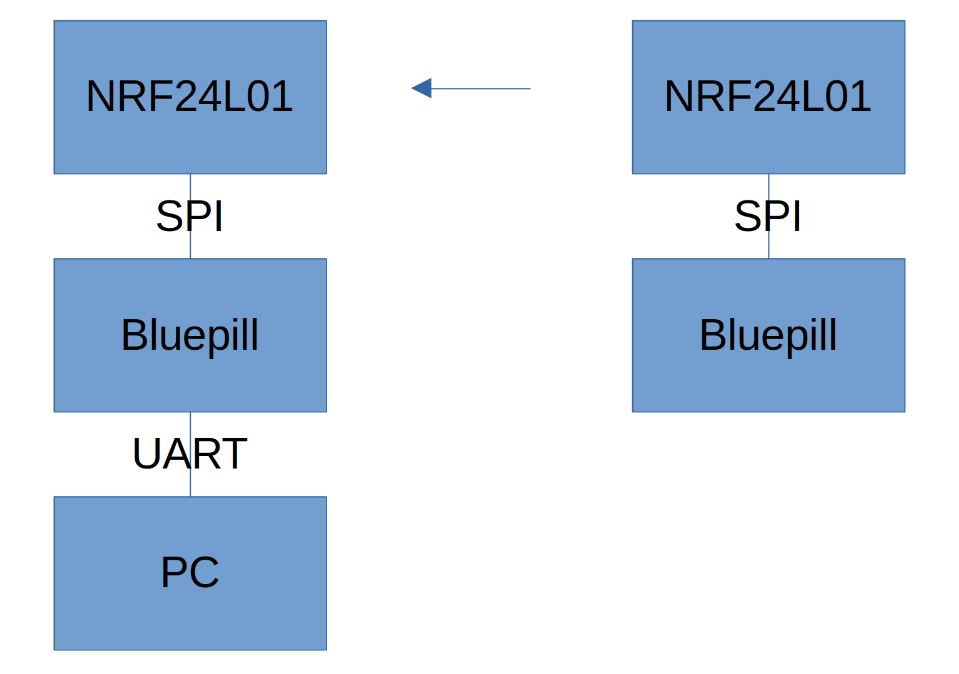
\includegraphics[width=0.5\textwidth]{Bloques.png}
    \caption{Diagrama en bloques del sistema propuesto.}
    \label{fig:SPI_write}
\end{figure}

\subsection{Arquitectura de archivos}

\begin{figure}[htbp]
    \centering
    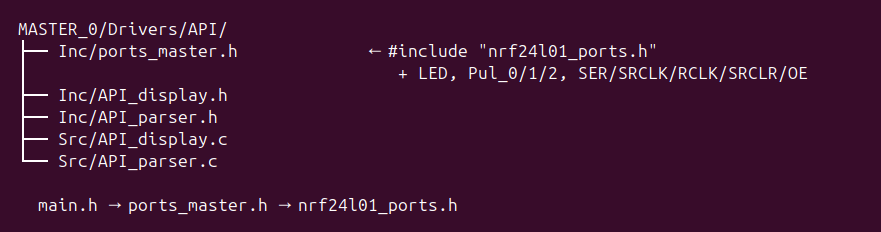
\includegraphics[width=0.75\textwidth]{Master_filesystem.png}
    \caption{Archivos en Master}
    \label{fig:files_master}
\end{figure}

\begin{figure}[htbp]
    \centering
    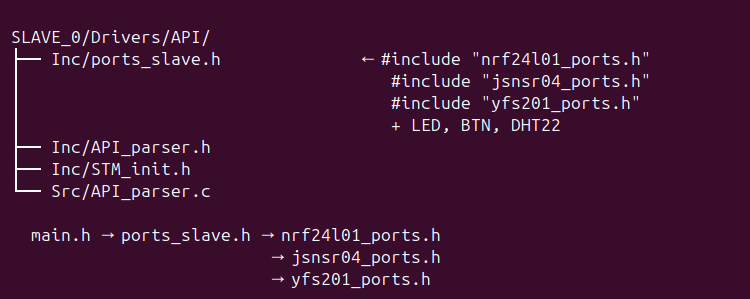
\includegraphics[width=0.75\textwidth]{Slave_filesystem.png}
    \caption{Archivos en slave}
    \label{fig:files_master}
\end{figure}

\begin{figure}[htbp]
    \centering
    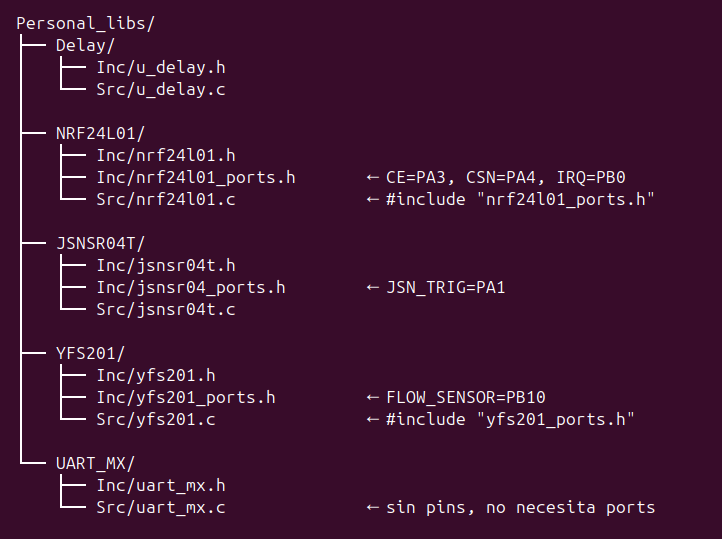
\includegraphics[width=0.75\textwidth]{PersonalLibs.png}
    \caption{Archivos en común, visibles entre maestro y esclavo}
    \label{fig:PersonalLIbs}
\end{figure}


Los archivos se acomodaron en la carpeta API, separados entre maestro y esclavo. Creé una carpeta Personal\_libs para portabilidad del código, donde cada librería tiene su propio archivo xxx\_ports.h con los defines de pines que usa. Los archivos ports\_master.h y ports\_slave.h actúan como agregadores: incluyen los ports de cada librería y definen los pines propios de cada nodo. El main.h generado por STM32CubeMX solo incluye el ports del nodo correspondiente dentro de la zona USER CODE, que CubeMX preserva ante regeneraciones.

\section{Delay}

El módulo JSNSR04T requiere un pulso de 10 uS, por ello tuve que generar un nuevo tipo de delay. 

La implementación de las funciones de temporización se encuentra en el archivo:
\href{https://github.com/matutecno/PdM_workspace_Matias_Morales/blob/36632c7629ba2d8375b50d48365e32dbffeaf255/TPF/Personal_libs/Delay/Src/u_delay.c#L17}{u\_delay.c (línea 17)}.

Por ello utilicé otro enfoque. DWT: Data watchpoint and trace. Habilitando el bit TRCENA (trace enable) en el registro de control de monitoreo y depuración del micro, habilita un contador de ciclos DWT. Esto lo que termina haciendo es contar la cantidad de ciclos de reloj por los que pasó el microcontrolador. De esta forma, si el microcontrolador está seteado con el PLL para trabajar a una frecuencia de 72 MHz, cada 72 flancos de clock tendremos un micro segundo (Esto se ve en la línea SystemCoreClock / 1000000U). La lógica de funcionamiento es idéntica a la implementada en clases, con start, running y duration.


\section{Transceptor nRF24L01}

El \textbf{nRF24L01} es un transceptor monolítico de radiofrecuencia (RF) que opera en la banda ISM (\textit{Industrial, Scientific, and Medical}) de $2.4$~GHz. Diseñado por \textit{Nordic Semiconductor}, este módulo destaca por su bajísimo consumo energético y su motor de protocolos acelerado por hardware, denominado \textbf{Enhanced ShockBurst™}.

\subsection{Características Principales}

\begin{description}
    \item[Banda de Operación:] $2.400$ a $2.525$~GHz ($125$ canales seleccionables).
    \item[Velocidad de Transmisión:] Configurable entre $250$~kbps, $1$~Mbps y $2$~Mbps.
    \item[Interfaz de Comunicación:] SPI (\textit{Serial Peripheral Interface}) de hasta $10$~Mbps.
    \item[Consumo de Energía:] Extremadamente bajo (aprox. $11.3$~mA en transmisión a $0$~dBm y $13.5$~mA en recepción a $2$~Mbps).
    \item[Tolerancia de Voltaje:] Alimentación de $1.9$ a $3.6$~V, con pines de entrada tolerantes a $5$~V, facilitando la interfaz con diversas familias de microcontroladores.
\end{description}

\subsection{Ventajas para el Proyecto}

\begin{itemize}
    \item \textbf{Gestión de Paquetes Automática:} El hardware gestiona el preámbulo, la dirección y la verificación de redundancia cíclica (CRC), reduciendo la carga computacional del microcontrolador STM32.
    \item \textbf{MultiCeiver™:} Capacidad de recibir datos de hasta seis nodos diferentes simultáneamente en topología estrella, lo cual simplifica la expansión futura del ecosistema domótico.
    \item \textbf{Dimensiones Reducidas:} Su factor de forma compacto permite una integración eficiente en el diseño de los PCB personalizados realizados en KiCad.
\end{itemize}


\section{Sensor de Ultrasonido Impermeable JSN-SR04T}

El \textbf{JSN-SR04T} es un transductor ultrasónico de distancia diseñado para aplicaciones que requieren resistencia a condiciones ambientales adversas. A diferencia de los sensores piezoeléctricos convencionales, este dispositivo cuenta con un transductor estanco y un cable de extensión (típicamente de $2.5$~metros), lo que permite separar la etapa de procesamiento electrónico del punto de medición.

\subsection{Especificaciones Técnicas}

El sensor presenta un rendimiento robusto bajo las siguientes características nominales:

\begin{table}[htbp]
    \centering
    \caption{Parámetros operativos del JSN-SR04T.}
    \label{tab:specs_jsnsr04}
    \begin{tabular}{@{}ll@{}}
        \toprule
        \textbf{Parámetro} & \textbf{Valor Nominal} \\ \midrule
        Tensión de operación & $3.0$~V a $5.5$~V DC \\
        Corriente de trabajo & $< 30$~mA \\
        Frecuencia acústica  & $40$~kHz \\
        Rango de medición    & $20$~cm a $600$~cm \\
        Resolución           & $1$~cm \\
        Ángulo de apertura   & $< 75^{\circ}$ \\ \bottomrule
    \end{tabular}
\end{table}

\subsection{Principio de Funcionamiento}

El dispositivo opera bajo el principio de \textit{Time of Flight} (ToF), calculando la distancia en función del tiempo transcurrido entre la emisión de una ráfaga sónica y la recepción de su eco. El ciclo de medición se describe mediante la siguiente secuencia:

\begin{enumerate}
    \item \textbf{Disparo (Trigger):} Se aplica un pulso de nivel alto (\textit{High}) de al menos $10~\mu$s en el pin \texttt{TRIG}.
    \item \textbf{Emisión:} El sensor emite automáticamente una ráfaga de ocho pulsos a $40$~kHz.
    \item \textbf{Respuesta (Echo):} El pin \texttt{ECHO} se activa en nivel alto. La duración de este pulso ($\Delta t$) es proporcional a la distancia recorrida por la onda.
\end{enumerate}

La distancia final se determina mediante la ecuación cinemática, considerando la velocidad del sonido ($v \approx 0.0343$~cm/us):

\begin{equation}
    d = \frac{\Delta t \times v}{2}
\end{equation}


\section{Periféricos utilizados}

\subsection{Interfaz SPI}                                                                                                                                                                                                                                      
                                                                                                                                                                                                                                                                                                                                                                                                                                                                                                                     
Ambos nodos del sistema —\textsc{Slave\_0} y \textsc{Master\_0}— utilizan el periférico \texttt{SPI1} del microcontrolador STM32F103C8T6 para comunicarse con el módulo de radio nRF24L01+. El bus opera en modo \textit{Full-Duplex Master}, con el        
  \textsc{stm32} como maestro y el nRF como esclavo único. La selección del esclavo se realiza por software mediante el pin \texttt{CSN} (chip select negado), controlado manualmente desde el driver.                                                        
                                                                                                                                                                                                                                                              
  El nRF24L01+ requiere adicionalmente un pin \texttt{CE} (\textit{Chip Enable}) para controlar los estados operativos de transmisión y recepción. Este pin no forma parte del bus SPI sino que es una señal de control independiente manejada por GPIO.      
                                                                                                                                                                                                                                                              
  \subsection{Configuración hardware}                                                                                                                                                                                                                         
                                                                                                                                                                                                                                                              
  Los pines asignados al bus SPI1 son idénticos en ambos nodos:                                                                                                                                                                                               
                                                                                                                                                                                                                                                              
  \begin{table}[h]                                                                                                                                                                                                                                            
  \centering                                                                                                                                                                                                                                                  
  \begin{tabular}{llll}                                                                                                                                                                                                                                       
  \hline                                                                                                                                                                                                                                                      
  \textbf{Pin} & \textbf{Señal} & \textbf{Dirección} & \textbf{Función} \\                                                                                                                                                                                    
  \hline                                                                                                                                                                                                                                                      
  PA3 & NRF\_CE    & Salida & Control de modo TX/RX \\                                                                                                                                                                                                        
  PA4 & NRF\_CSN   & Salida & Chip Select (activo en bajo) \\                                                                                                                                                                                                 
  PA5 & SPI1\_SCK  & Salida & Reloj SPI \\                                                                                                                                                                                                                    
  PA6 & SPI1\_MISO & Entrada & Datos maestro $\leftarrow$ esclavo \\                                                                                                                                                                                          
  PA7 & SPI1\_MOSI & Salida & Datos maestro $\rightarrow$ esclavo \\                                                                                                                                                                                          
  PB0 & NRF\_IRQ   & Entrada & Interrupción (EXTI, flanco descendente) \\                                                                                                                                                                                     
  \hline                                                                                                                                                                                                                                                      
  \end{tabular}                                                                                                                                                                                                                                               
  \caption{Pinout SPI y control nRF24L01+ (idéntico en ambos nodos)}                                                                                                                                                                                          
  \end{table}                                                                                                                                                                                                                                                 
  
  Los parámetros del periférico configurados en STM32CubeMX son:                                                                                                                                                                                              
  
  \begin{itemize}                                                                                                                                                                                                                                             
      \item \textbf{Modo:} Full-Duplex Master
      \item \textbf{Polaridad de reloj (CPOL):} 0 — reposo en bajo                                                                                                                                                                                            
      \item \textbf{Fase de reloj (CPHA):} 0 — muestreo en flanco ascendente (Modo 0)                                                                                                                                                                         
      \item \textbf{Prescaler:} /8 → frecuencia de reloj: $\frac{72\,\text{MHz}}{8} = 9\,\text{MHz}$                                                                                                                                                          
      \item \textbf{NSS:} software (control manual por GPIO)                                                                                                                                                                                                  
      \item \textbf{DMA:} DMA1 canal 2 (SPI1\_RX), DMA1 canal 3 (SPI1\_TX)                                                                                                                                                                                    
  \end{itemize}                                                                                                                                                                                                                                               
                                                                                                                                                                                                                                                              
  \subsection{Driver nRF24L01+}                                                                                                                                                                                                                               

  El driver fue desarrollado como biblioteca personal compartida entre ambos nodos, ubicada en \texttt{Personal\_libs/NRF24L01/}. Toda comunicación con el módulo se realiza a través de \texttt{HAL\_SPI\_TransmitReceive\_DMA}, aprovechando el modo        
  full-duplex: cada transacción envía un comando por MOSI y recibe simultáneamente la respuesta por MISO.
                                                                                                                                                                                                                                                              
                                                                                                                                                                                                                                                              
  \subsubsection{Sincronización con DMA}                                                                                                                                                                                                                      
  
  La transferencia es no bloqueante: el DMA mueve los datos de forma autónoma y, al completarse, dispara la interrupción que ejecuta el callback:                                                                                                             
  
  \begin{verbatim}                                                                                                                                                                                                                                            
  void HAL_SPI_TxRxCpltCallback(SPI_HandleTypeDef *hspi) {
      csnHigh();                                                                                                                                                                                                                                              
      _busy = false;
  }                                                                                                                                                                                                                                                           
  \end{verbatim}                                                                                                                                                                                                                                              
  
  El flag \texttt{\_busy} (declarado \texttt{volatile}) sincroniza el estado del bus entre el hilo principal y el contexto de interrupción. Para evitar bloqueos ante fallas del DMA —situación detectada durante el desarrollo donde                         
  \texttt{HAL\_SPI\_TransmitReceive\_DMA} devolvía \texttt{HAL\_BUSY} ocasionalmente—, se implementó la función \texttt{\_waitBusy()} con timeout basado en el contador DWT:
                                                                                                                                                                                                                                                              
  \begin{verbatim}
  static void _waitBusy(void) {
      delayUsSet(&del_TIMEOUT, TIMEOUT);    /* TIMEOUT = 100 µs */
      while (_busy && !delayUsRead(&del_TIMEOUT)) {}                                                                                                                                                                                                          
      if (_busy) {                                                                                                                                                                                                                                            
          _busy = false;                                                                                                                                                                                                                                      
          csnHigh();                                                                                                                                                                                                                                          
      }
  }                                                                                                                                                                                                                                                           
  \end{verbatim}
                                                                                                                                                                                                                                                              
  Si el DMA no libera el bus en 100\,µs, el driver recupera el estado manualmente elevando \texttt{CSN} y limpiando el flag.                                                                                                                                  La idea fue implementar una suerte de watchdog para el periférico. 
  
\textbf{  Observación:} Si bien se observó una mejoría de la estabilidad del sistema con esta implementación, actualmente estoy lidiando con un problema en los módulos. Al iniciar el slave, algunas veces no transmite información y el sistema 'cuelga'. Hay que reiniciar manualmente para que inicie. Sospecho de una fuente de alimentación inestable (3v3 generados con un ams1117, con capacitores de 100 nF SMD y 470 uF electrolíticos). El próximo paso a probar es implementar un módulo step down para ver de solucionar esto.
  
  \subsubsection{Funciones de acceso al bus}                                                                                                                                                                                                                  
  
  \begin{itemize}                                                                                                                                                                                                                                             
      \item \texttt{nrfWriteReg(reg, val)}: escribe un registro de 8 bits. Envía el comando \texttt{W\_REGISTER} (0x20 \texttt{|} reg) seguido del valor.
      \item \texttt{nrfReadReg(reg)}: lee un registro. Envía \texttt{R\_REGISTER} (0x00 \texttt{|} reg) y \texttt{NOP} (0xFF); el dato útil está en \texttt{\_rx\_buf[1]}.                                                                                    
      \item \texttt{nrfWriteAddr(reg, addr, len)}: escribe una dirección de hasta 5 bytes en un ciclo DMA único.                                                                                                                                              
      \item \texttt{nrfTransmit(data, len)}: carga el payload en la TX FIFO mediante el comando \texttt{W\_TX\_PAYLOAD} (0xA0), espera a que el DMA finalice y genera el pulso de \texttt{CE} ($\geq$10\,µs mínimo según datasheet, implementado con          
  \texttt{HAL\_Delay(1)}).                                                                                                                                                                                                                                    
      \item \texttt{nrfRecept(data, len)}: verifica el flag \texttt{RX\_DR} en el registro \texttt{STATUS}; si hay dato disponible, lo lee con el comando \texttt{R\_RX\_PAYLOAD} (0x61) y limpia el flag.                                                    
  \end{itemize}                                                                                                                                                                                                                                               
  
  \subsection{Configuración del módulo nRF24L01+}                                                                                                                                                                                                             

  Ambos nodos utilizan los mismos parámetros de radio. La tabla~\ref{tab:nrf_regs} resume la configuración de registros aplicada en la inicialización.                                                                                                        
  
  \begin{table}[h]                                                                                                                                                                                                                                            
  \centering
  \begin{tabular}{lllp{6.5cm}}
  \hline                                                                                                                                                                                                                                                      
  \textbf{Registro} & \textbf{Dir.} & \textbf{Valor} & \textbf{Configuración} \\
  \hline                                                                                                                                                                                                                                                      
  CONFIG     & 0x00 & 0x0E / 0x0F & PWR\_UP=1, CRC habilitado (1 byte); PRIM\_RX=0 (TX) / PRIM\_RX=1 (RX) \\                                                                                                                                                  
  EN\_AA     & 0x01 & 0x00        & Auto-acknowledge deshabilitado en todos los pipes \\                                                                                                                                                                      
  SETUP\_RETR & 0x04 & 0x00       & Sin retransmisiones (ARC=0) \\                                                                                                                                                                                            
  RF\_CH     & 0x05 & 0x64 (100)  & Canal 100 → 2500\,MHz \\                                                                                                                                                                                                  
  RF\_SETUP  & 0x06 & 0x06        & 1\,Mbps, potencia máxima (0\,dBm) \\                                                                                                                                                                                      
  RX\_PW\_P0 & 0x11 & 10          & Payload fijo de 10 bytes (\texttt{sizeof(payload\_t)}) \\                                                                                                                                                                 
  TX\_ADDR / RX\_ADDR\_P0 & 0x10/0x0A & \multicolumn{2}{l}{\texttt{\{0xEF, 0xEF, 0xEF, 0xEF, 0xEF\}} (5 bytes)} \\                                                                                                                                            
  \hline                                                                                                                                                                                                                                                      
  \end{tabular}                                                                                                                                                                                                                                               
  \caption{Registros del nRF24L01+ configurados en la inicialización}                                                                                                                                                                                         
  \label{tab:nrf_regs}
  \end{table}                                                                                                                                                                                                                                                 
  
  Por lo pronto, el sistema opera en modo \textit{fire-and-forget}: el transmisor no espera confirmación de recepción. Esta decisión simplifica el protocolo a costa de no garantizar la entrega de cada paquete individual.                                                 
  
  \subsection{Estructura del payload}                                                                                                                                                                                                                         
  
  La estructura de datos transmitida por SPI desde el \textsc{Slave} hacia el módulo nRF —y recibida por el \textsc{Master}— ocupa exactamente 10 bytes:                                                                                                      
  
  \begin{verbatim}                                                                                                                                                                                                                                            
  typedef struct {
      uint16_t nivel;        /* distancia en cm              */
      uint16_t caudal;       /* pulsos por segundo           */                                                                                                                                                                                               
      uint16_t luminosidad;  /* valor ADC raw (12 bits)      */
      int16_t  temperatura;  /* temperatura en °C × 10       */                                                                                                                                                                                               
      uint8_t  humedad;      /* humedad relativa en %        */
  } payload_t;                                                                                                                                                                                                                                                
  \end{verbatim}
  
  Esto se diseñó de esta forma para una posible modificación a futuro, teniendo ya prevista la trama en el caso de que se desee implementar algún otro tipo de sensor.
  
    \textbf{Observación: }  El padding al final existe para que, al ponerse dos payload\_t seguidos en un     
  array, el segundo también empiece en dirección par:                           

\begin{verbatim}

  payload\_t arr[2];                                                             
  // &arr[0] = 0x00  // par
  // &arr[1] = 0x0A  // par  (sin padding sería 0x09, impar -> problema)          
  
\end{verbatim}

                                                                                
  Por eso sizeof(payload\_t) == 10 y no 9. 
  
  \subsection{Uso del SPI en cada nodo}                                                                                                                                                                                                                       
  
  \paragraph{Slave\_0 (transmisor).}                                                                                                                                                                                                                          
  Inicializa el módulo en modo TX mediante \texttt{nrfSetModeTX()}. En cada ciclo de la FSM, una vez obtenida la medición del sensor JSN-SR04T, invoca \texttt{nrfTransmit()} para enviar la estructura \texttt{payload\_t} al Master. La FSM transita por los
   estados: \texttt{MEASURE} $\to$ \texttt{MEASURING} $\to$ \texttt{UART} $\to$ \texttt{NRF} $\to$ \texttt{WAITING} $\to$ \texttt{MEASURE}.                                                                                                                   
  
  \paragraph{Master\_0 (receptor).}                                                                                                                                                                                                                           
  Inicializa el módulo en modo RX mediante \texttt{nrfSetModeRX()}, con \texttt{CE} en alto de forma permanente. En cada ciclo de la FSM consulta \texttt{nrfRecept()} para verificar si hay un paquete disponible en la RX FIFO. Ante 10 segundos sin
  recepción, un watchdog por software pone \texttt{payload.nivel = 0} y actualiza el display. La FSM transita por: \texttt{RECEIVE} $\to$ \texttt{UART} $\to$ \texttt{PRINT\_LEV} $\to$ \texttt{RECEIVE}.                                                     
  
  Adicionalmente, al finalizar \texttt{initParser()}, el Master verifica que el registro \texttt{CONFIG} del nRF valga \texttt{0x0F}; en caso contrario ejecuta \texttt{NVIC\_SystemReset()} para forzar una reinicialización completa del sistema.           

\subsection{Interfaz UART}                                          
                                                                                
  Ambos nodos utilizan \texttt{USART1} del STM32F103C8T6 exclusivamente como    
  canal de telemetría hacia una terminal serie en PC. El periférico opera en
  modo transmisión únicamente (\textit{TX-only}); la recepción está implementada
   en el driver pero no se usa en la aplicación del TPF.

  \subsection{Configuración hardware}

  \begin{table}[h]                                                              
  \centering
  \begin{tabular}{llll}                                                         
  \hline
  \textbf{Pin} & \textbf{Señal} & \textbf{Dirección} & \textbf{Función} \\
  \hline
  PA9  & USART1\_TX & Salida  & Transmisión de datos hacia PC \\
  PA10 & USART1\_RX & Entrada & Recepción (configurado, no utilizado) \\        
  \hline                                                                        
  \end{tabular}                                                                 
  \caption{Pinout UART1 (idéntico en ambos nodos)}                              
  \end{table}                                                                   
  
  Parámetros configurados en STM32CubeMX:                                       

  \begin{itemize}                                                               
      \item \textbf{Baud rate:} 115200 bps
      \item \textbf{Trama:} 8 bits de datos, sin paridad, 1 bit de stop (8N1)   
      \item \textbf{DMA TX:} DMA1 canal 4 (\texttt{USART1\_TX})                 
  \end{itemize}
  
  \textbf{Observación: }El GPIO en TX RX se encuentra protegido con un resistor de 330 ohms para proteger al gpio ante un corto circuito accidental. El handler para UART se implementó al setear STMCubeMx, por lo que no fue necesario realizar la configuración hecha en clases.
                                                                                
  \subsection{Driver UART\_MX}

  El driver fue desarrollado como biblioteca personal compartida entre ambos    
  nodos, ubicada en \texttt{Personal\_libs/UART\_MX/}. Abstrae el
  \texttt{UART\_HandleTypeDef} generado por CubeMX y expone una API de alto     
  nivel independiente del periférico concreto.

  El header incluye guards de compilación condicional para soportar tanto la    
  familia STM32F1 como STM32F4:
                                                                                
  \begin{verbatim}
  #if defined(STM32F446xx)
      #include "stm32f4xx_hal.h"
  #elif defined(STM32F103xB)
      #include "stm32f1xx_hal.h"
  #endif
  \end{verbatim}

  \subsubsection{Inicialización}                                                
  
  \begin{verbatim}                                                              
  bool uartInit(UART_HandleTypeDef *uart);
  \end{verbatim}

  Almacena el puntero al handle en una variable estática de módulo y inicializa 
  el timer de timeout interno. Devuelve \texttt{false} si el puntero es
  \texttt{NULL}.                                                                

  \subsubsection{Transmisión}

  \begin{verbatim}
  void uartSendString(uint8_t *pstring);
  \end{verbatim}                                                                
  
  Espera a que el periférico quede en estado \texttt{HAL\_UART\_STATE\_READY}   
  antes de lanzar la transferencia mediante \texttt{HAL\_UART\_Transmit\_DMA()}.
   Para evitar bloqueos indefinidos ante fallas del bus, la espera tiene un     
  timeout de 10\,ms implementado con el contador DWT:

  \begin{verbatim}
  delayUsSet(&del_uart, TIMEOUT);   /* TIMEOUT = 10000 µs = 10 ms */
  while (UartHandle->gState != HAL_UART_STATE_READY                             
         && !delayUsRead(&del_uart));
  HAL_UART_Transmit_DMA(UartHandle, pstring, strlen((char*)pstring));           
  \end{verbatim}
  
  Esto también busca de funcionar como un watch dog.
                                                                                
  La longitud de la cadena se calcula en tiempo de ejecución con                
  \texttt{strlen()}, por lo que la cadena debe estar terminada en
  \texttt{'\textbackslash 0'}.                                                  

  \subsubsection{Recepción}

  \begin{verbatim}
  int8_t uartReceiveString(uint8_t *pstring);
  \end{verbatim}                                                                
  
  Lee caracteres de a uno usando \texttt{HAL\_UART\_Receive()} con timeout de   
  1\,ms por carácter, acumulando en un buffer estático interno. Retorna
  \texttt{1} cuando detecta \texttt{'\textbackslash n'} o                       
  \texttt{'\textbackslash r'}, \texttt{0} si no llegó ningún carácter en el
  timeout, y \texttt{-1} ante overflow (límite: \texttt{CMD\_MAX\_LINE = 64}
  bytes). Esta función no se utiliza en la aplicación actual del TPF.

  \subsection{Uso en cada nodo}

  \paragraph{Slave\_0.}                                                         
  Transmite una línea por cada medición del sensor JSN-SR04T, en el estado
  \texttt{UART} de la FSM:                                                      
  \begin{verbatim}
  snprintf(buf, sizeof(buf), "Medicion: %u cm \r\n", med);                      
  uartSendString(buf);                                                          
  \end{verbatim}
                                                                                
  \paragraph{Master\_0.}
  Transmite el valor recibido por radio en el estado \texttt{UART} de la FSM,
  junto con mensajes de diagnóstico al arranque (\texttt{``Sistema online''} y  
  volcado de registros del nRF):
  \begin{verbatim}                                                              
  snprintf(buff, sizeof(buff), "\nMedicion: %u \r", payload.nivel);
  uartSendString(buff);
  \end{verbatim}                                                                
  
  En ambos casos el buffer de transmisión es local a la FSM (32 bytes),         
  formateado con \texttt{snprintf()} antes de cada envío.


\section{Arquitectura del hardware}

El sistema se divide en dos unidades funcionales con las siguientes características:

\textbf{Nodo transmisor: }

\begin{itemize}
	\item \textbf{Unidad de Procesamiento:} Microcontrolador STM32F103C8T6 (Blue Pill).
	\item \textbf{Interfaz de Radio:} Módulo nRF24L01 conectado mediante bus SPI.
	\item \textbf{Sensores:} Entrada para sensor ultrasónico JSN-SR04T (impermeable) para medición de nivel/distancia.
\end{itemize}

\textbf{Nodo receptor}

\begin{itemize}
	\item \textbf{Unidad de Procesamiento:} Microcontrolador STM32F103C8T6 (Blue Pill).
	\item \textbf{Interfaz de Radio:} Módulo nRF24L01 (SPI).
	\item \textbf{Interfaz de Usuario/PC:} Comunicación via UART hacia una PC para la visualización de datos mediante un terminal serie o interfaz gráfica.
	\item \textbf{Indicadores luminosos y sonoros:} Implementación de un display de segmentos verticales para indicar nivel y buzzer de alarma sonora.
\end{itemize}

Se adjuntan los esquemáticos del hardware implementado en la carpeta del trabajo final, tanto del master como del slave. Como punto a destacar, se observa el uso de resistores a la salida del gpio para proteger las salidas. En los casos de las señales a 5v, se utilizó un zenner de 3v3 como adaptador de tensión para el gpio. En el master, se observa el uso de un registro de desplazamiento como driver para los leds, mediante el uso de un 74hc595.

\begin{figure}[htbp]
    \centering
    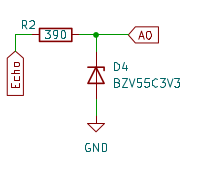
\includegraphics[width=0.35\textwidth]{zenner.png}
    \caption{Protecciones y adaptaciones de voltajes para el GPIO.}
    \label{fig:zenner}
\end{figure}

\begin{figure}[htbp]
    \centering
    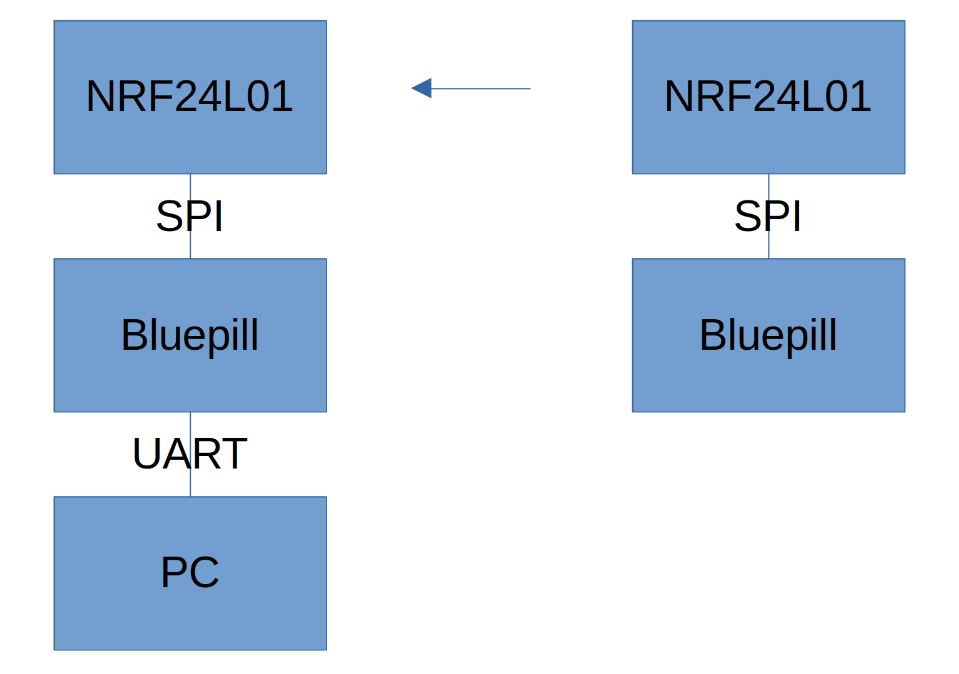
\includegraphics[width=0.5\textwidth]{Bloques.png}
    \caption{Diagrama en bloques del sistema propuesto.}
    \label{fig:Bloq}
\end{figure}

\begin{figure}[htbp]
    \centering
    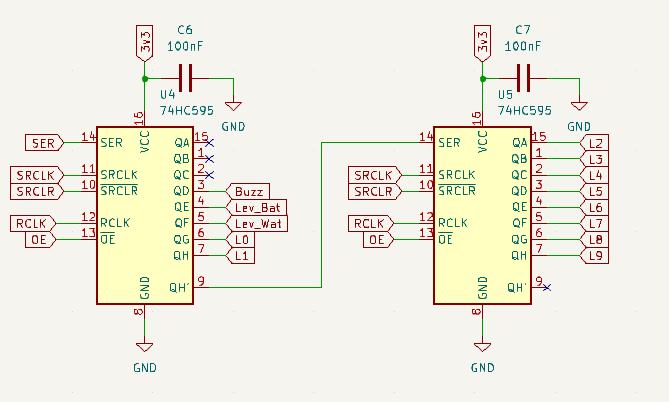
\includegraphics[width=0.5\textwidth]{shift_reg.png}
    \caption{Interconexión entre registros de desplazamiento.}
    \label{fig:shift_reg}
\end{figure}

\begin{figure}[htbp]
    \centering
    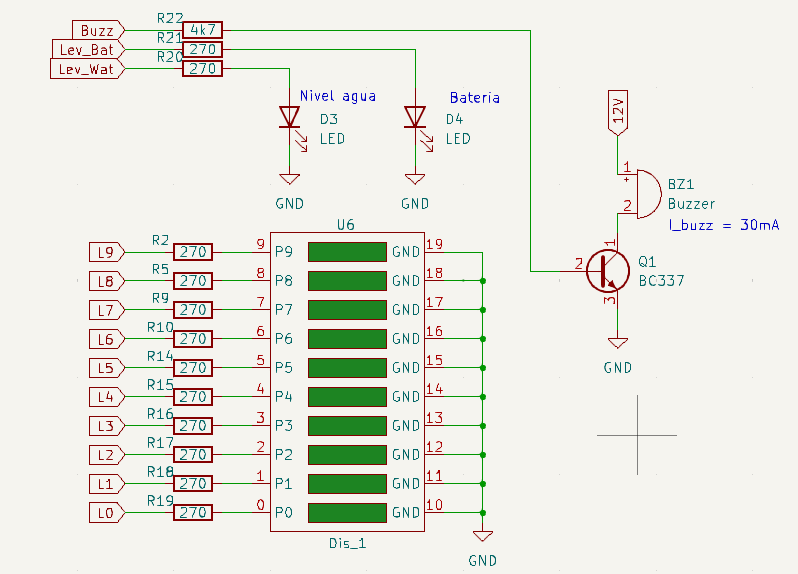
\includegraphics[width=0.5\textwidth]{Leds.png}
    \caption{Sistema display implementado.}
    \label{fig:Leds}
\end{figure}

\begin{figure}[htbp]
    \centering
    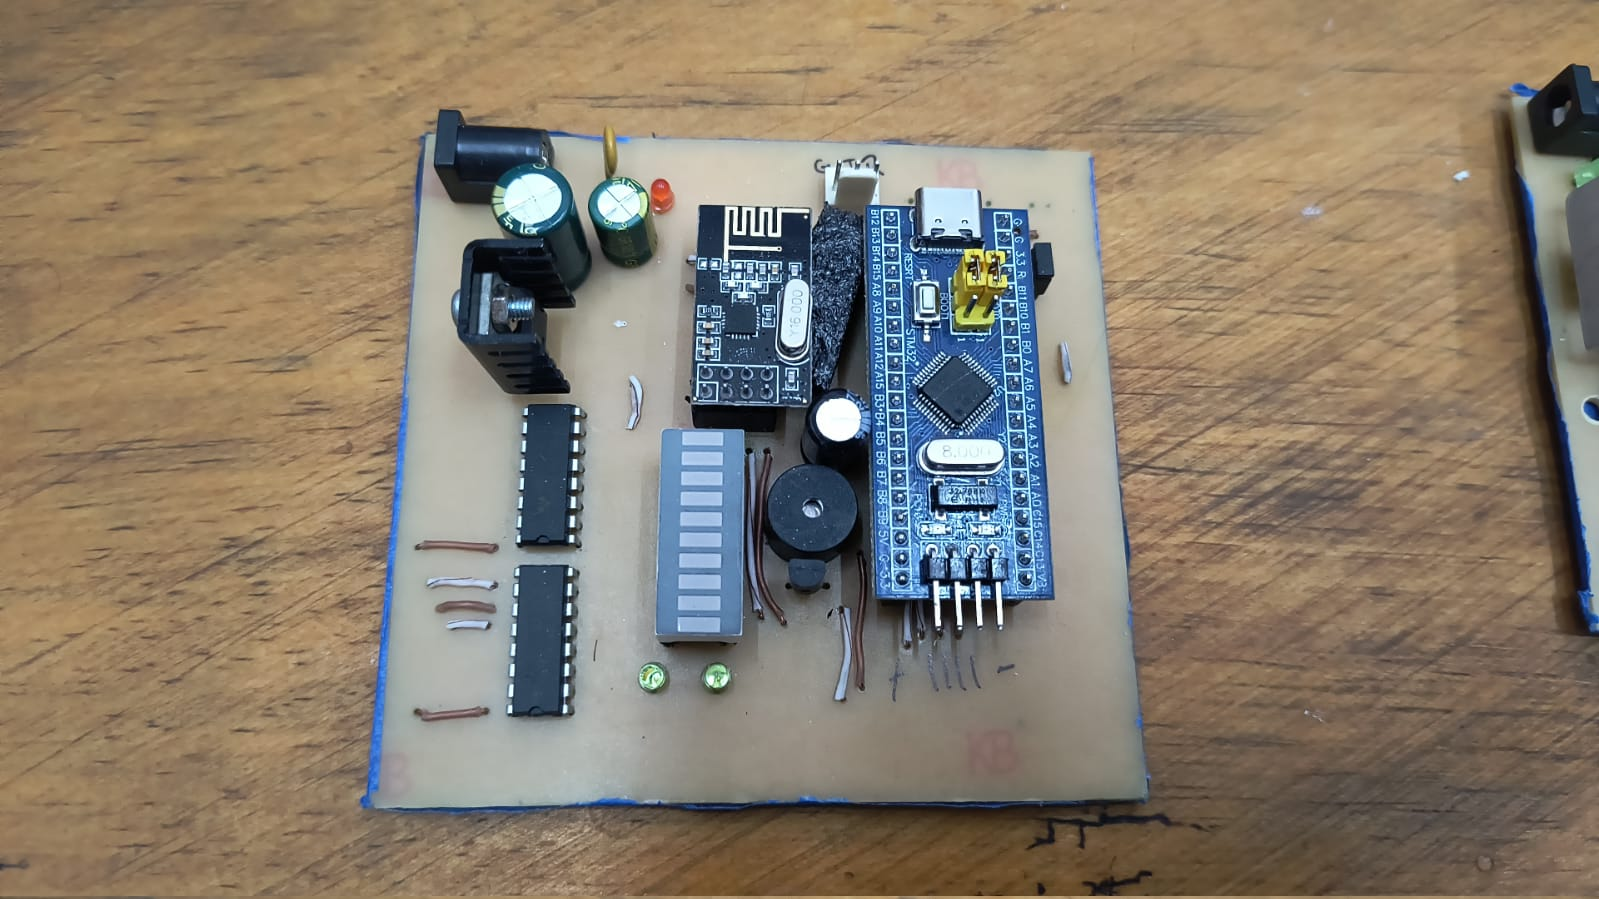
\includegraphics[width=0.5\textwidth]{Master.jpeg}
    \caption{Circuito Master.}
    \label{fig:Master}
\end{figure}

\begin{figure}[htbp]
    \centering
    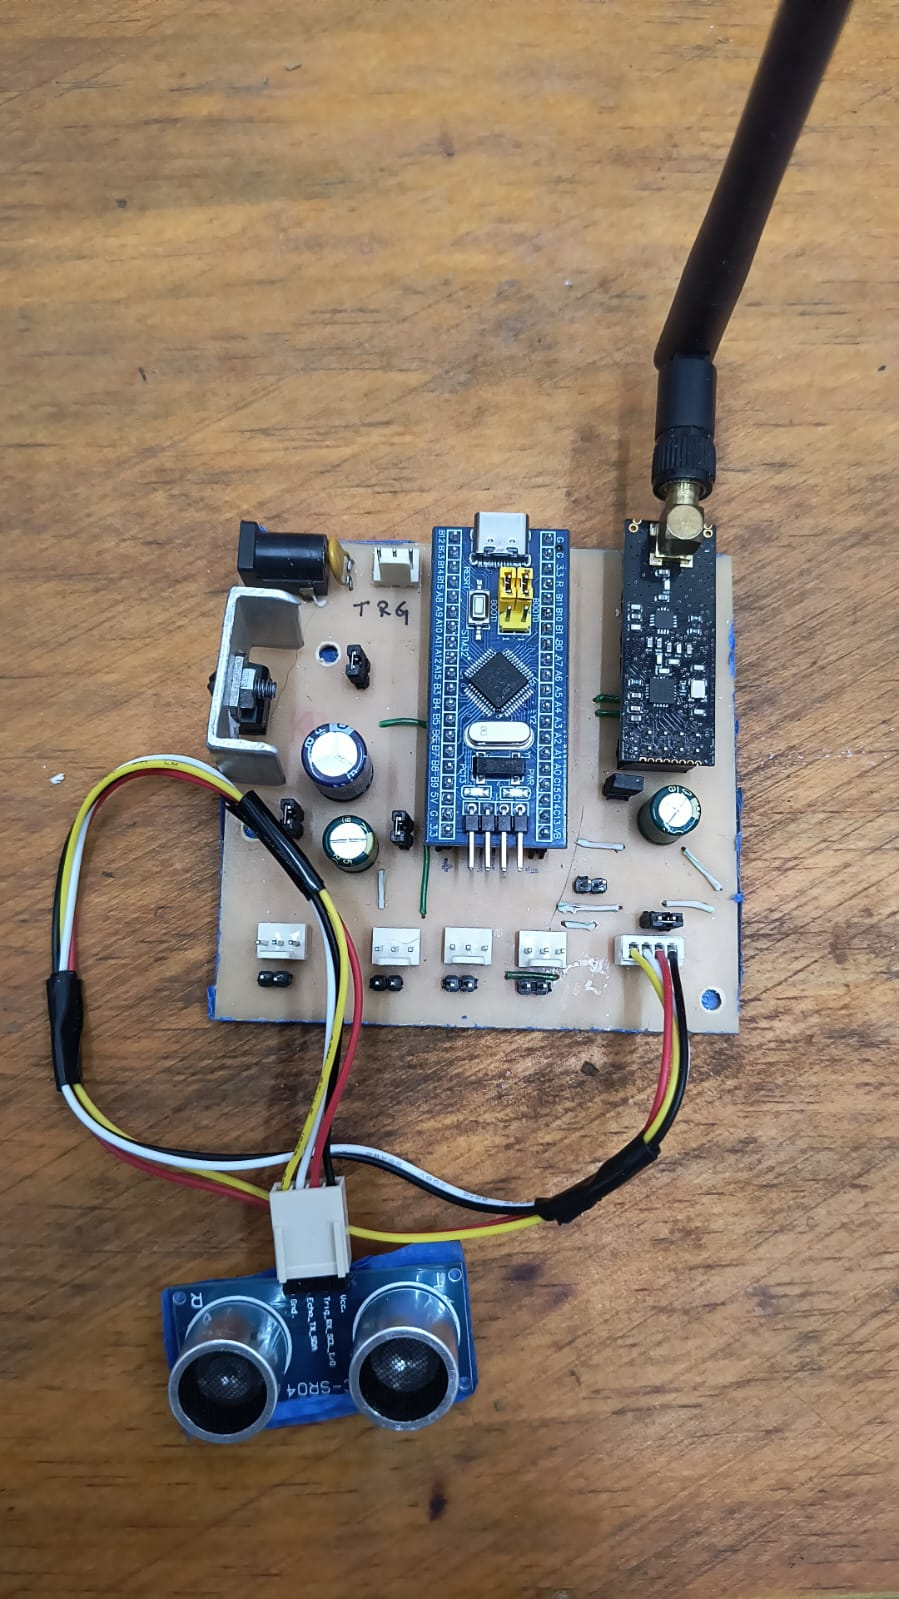
\includegraphics[width=0.35\textwidth]{Slave.jpeg}
    \caption{Circuito Slave.}
    \label{fig:Slave}
\end{figure}

La lógica de control de la pantalla se encuentra definida en el archivo 
\href{https://github.com/matutecno/PdM_workspace_Matias_Morales/blob/36632c7629ba2d8375b50d48365e32dbffeaf255/TPF/Master_0/Master_0/STM32CubeIDE/Drivers/API/Src/API_display.c#L124}{API\_display.c (línea 124)}. Se implementó un código similar a la función shiftOut(), conocida de Arduino. En resumen, lo que hace es transformar una trama de datos en una trama sincrónica. 

\section{Máquinas de estado}

\begin{figure}[htbp]
    \centering
    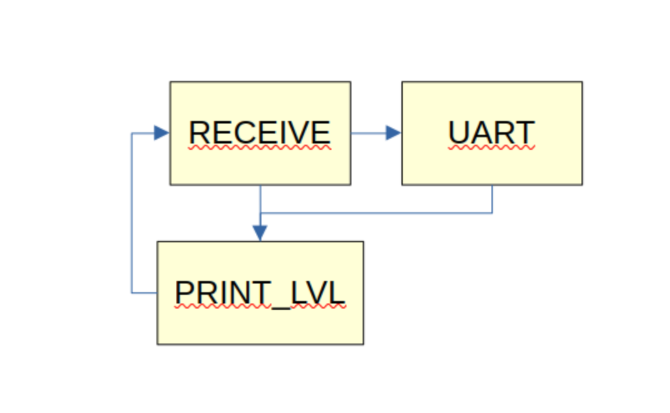
\includegraphics[width=0.5\textwidth]{ST_MASTER.png}
    \caption{Máquina de estados del master.}
    \label{fig:st_master}
\end{figure}


\begin{figure}[htbp]
    \centering
    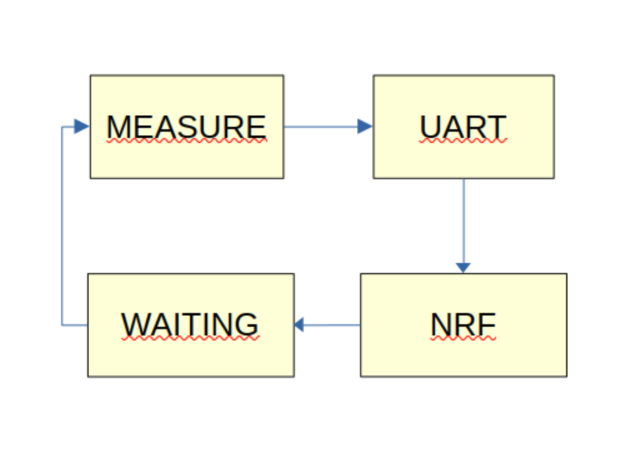
\includegraphics[width=0.5\textwidth]{ST_SLAVE.png}
    \caption{Máquina de estados del slave.}
    \label{fig:st_slave}
\end{figure}

\section{Ejemplo de variables globales privadas}

Un ejemplo claro de este uso lo vemos en la variable de las máquinas de estado:

\href{https://github.com/matutecno/PdM_workspace_Matias_Morales/blob/36632c7629ba2d8375b50d48365e32dbffeaf255/TPF/SLAVE_0/Slave_0/STM32CubeIDE/Drivers/API/Src/API_parser.c#L25}{Variable global estática FMS - Slave}

\section{Actualización FSM - Master y slave}

Se adjuntan las primeras líneas de actualización de las máquinas de estado, tanto del master como del slave.

\href{https://github.com/matutecno/PdM_workspace_Matias_Morales/blob/36632c7629ba2d8375b50d48365e32dbffeaf255/TPF/SLAVE_0/Slave_0/STM32CubeIDE/Drivers/API/Src/API_parser.c#L49}{Update FSM slave}

\href{https://github.com/matutecno/PdM_workspace_Matias_Morales/blob/36632c7629ba2d8375b50d48365e32dbffeaf255/TPF/Master_0/Master_0/STM32CubeIDE/Drivers/API/Src/API_parser.c#L50}{Update FSM Master}

\section{The power of 10 rules}

\begin{itemize}
	\item \textbf{Sin goto ni recursiones: }Cumple.
	\item \textbf{Bucles con límites fijos: }Todos los while tienen salida por  timeout DWT.
	\item \textbf{Sin memoria dinámica:} No hay malloc, calloc ni free en ningún módulo.
	\item \textbf{Funciones de una página:} Cumpel en general. 
	\item \textbf{Mínima visibilidad:} Cumple. Todas las variables son static.
	\item \textbf{Preprocesador moderado:} Cumple. Solo se usa para constantes.
	\item \textbf{Punteros con una sola referencia:} Cumple. No hay punteros a punteros ni cadenas de desreferencias (-> de un solo nivel).
	\item \textbf{Sin punteros a funciones:} Cumple. No hay punteros a funciones en ningún módulo.
\end{itemize}

\section{Ejemplos comentarios en líneas}

\href{https://github.com/matutecno/PdM_workspace_Matias_Morales/blob/36632c7629ba2d8375b50d48365e32dbffeaf255/TPF/Master_0/Master_0/STM32CubeIDE/Drivers/API/Src/API_parser.c#L58}{Línea explicativa}

\href{https://github.com/matutecno/PdM_workspace_Matias_Morales/blob/36632c7629ba2d8375b50d48365e32dbffeaf255/TPF/Master_0/Master_0/STM32CubeIDE/Drivers/API/Src/API_parser.c#L46}{Línea explicativa}

\href{https://github.com/matutecno/PdM_workspace_Matias_Morales/blob/36632c7629ba2d8375b50d48365e32dbffeaf255/TPF/Master_0/Master_0/STM32CubeIDE/Drivers/API/Src/API_display.c#L18}{Línea explicativa}

\subsection{Escalabilidad y Visión de Futuro}

El diseño del sistema se ha concebido bajo un paradigma de \textbf{arquitectura modular}, permitiendo su integración como un nodo periférico dentro de un ecosistema de domótica más robusto. 

Al emplear el estándar de comunicaciones nRF24L01+, el sistema queda preparado para:
\begin{itemize}
    \item \textbf{Topología de Red:} Evolucionar de un enlace punto a punto hacia una red tipo estrella o malla (Mesh), integrando múltiples nodos sensores distribuidos en una vivienda o planta industrial.
    \item \textbf{Interoperabilidad:} Actuar como un \textit{gateway} inalámbrico que, mediante la interfaz UART de la unidad central, pueda conectarse a plataformas de control de nivel superior como \textit{Home Assistant}, \textit{OpenHAB} o servidores MQTT sobre una Raspberry Pi.
    \item \textbf{Modularidad de Hardware:} La separación de las etapas de potencia (control de cargas como el lavarropas) y las etapas de lógica asegura que el módulo pueda adaptarse a diferentes aplicaciones domésticas sin requerir un rediseño del núcleo de procesamiento.
\end{itemize}







\end{document}